\chapter{Applicatie}
\label{ch:applicatie}

\section{Gebruikte Software}
Het product werd gerealiseerd met behulp van de game engine Unity3d. Dit was een zeer fijne tool om te gebruiken aangezien de integratie met de Oculus Go zeer goed is verwerkt in het programma. Na het downloaden van de Oculus Integration package kon men vrijwel meteen aan de slag ermee. Ook werd er gebruik gemaakt van de Unity Asset store. Deze store bevat heel wat (gratis) 3D modellen, geluidseffecten, animaties, etc.

\section{Gerealiseerde product}
Het gerealiseerde product is een game waar de gebruiker in een virtuele omgeving terecht komt. Hier kan hij met behulp van de controllers fictieve appels plukken uit bomen en ze in de juiste mand leggen. Bij het uitschrijven van het idee voor de applicatie werd er vooral gefocust op één bepaalde beweging waar men van beneden gecontroleerd naar boven dient te reiken en opnieuw naar beneden. De applicatie richt zich dan vooral ook op de revalidatie van de bovenste ledematen.

\section{Mogelijke features voor in de toekomst}
Momenteel is de applicatie nog puur een proof of concept maar deze zou in de toekomst eventueel nog verder uitgewerkt kunnen worden. Men zou bijvoorbeeld verschillende levels kunnen toevoegen die elk focussen op een andere beweging. Voorlopig is er ook nog geen score-systeem wat het spel toch zeker uitdagender zou maken. Daarnaast zou het ook zeer interessant zijn voor de kinesist om wat gegevens op te kunnen vragen van de patiënt of hij zijn bewegingen heeft gedaan, of er vorderingen zijn, etc.

\begin{figure}[p]
    \centering
    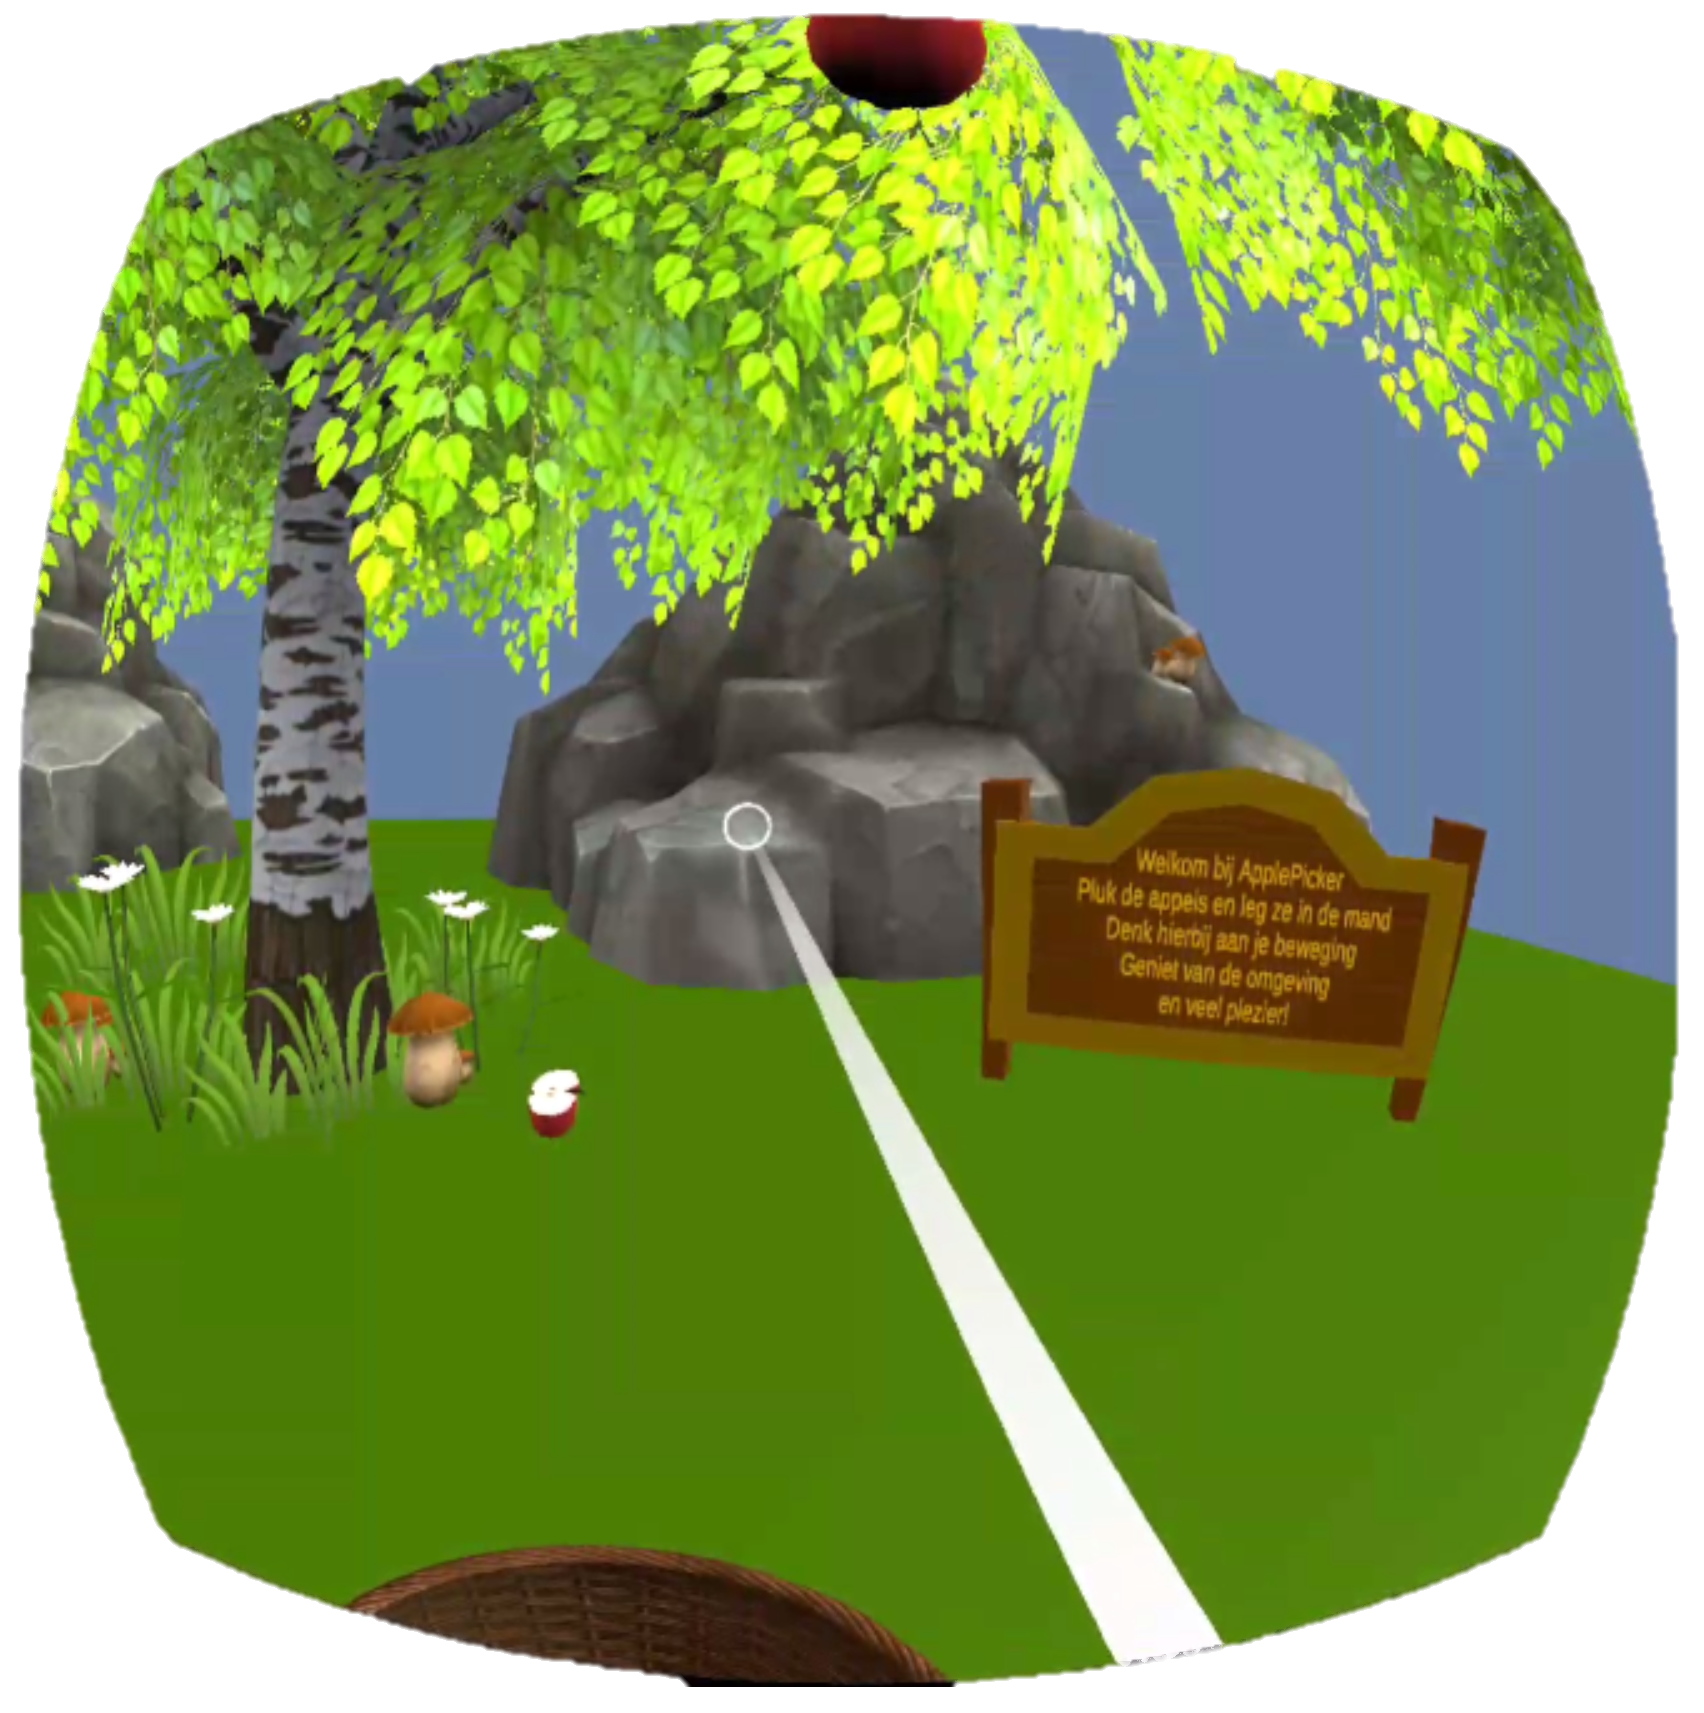
\includegraphics[scale=0.5]{apple1.png}
    \caption{ApplePicker screenshot welkomstbord}
\end{figure}

\begin{figure}[h]
    \centering
    \includegraphics[scale=0.5]{apple2.png}
    \caption{ApplePicker screenshot appels in de boom}
\end{figure}

\begin{figure}[h]
    \centering
    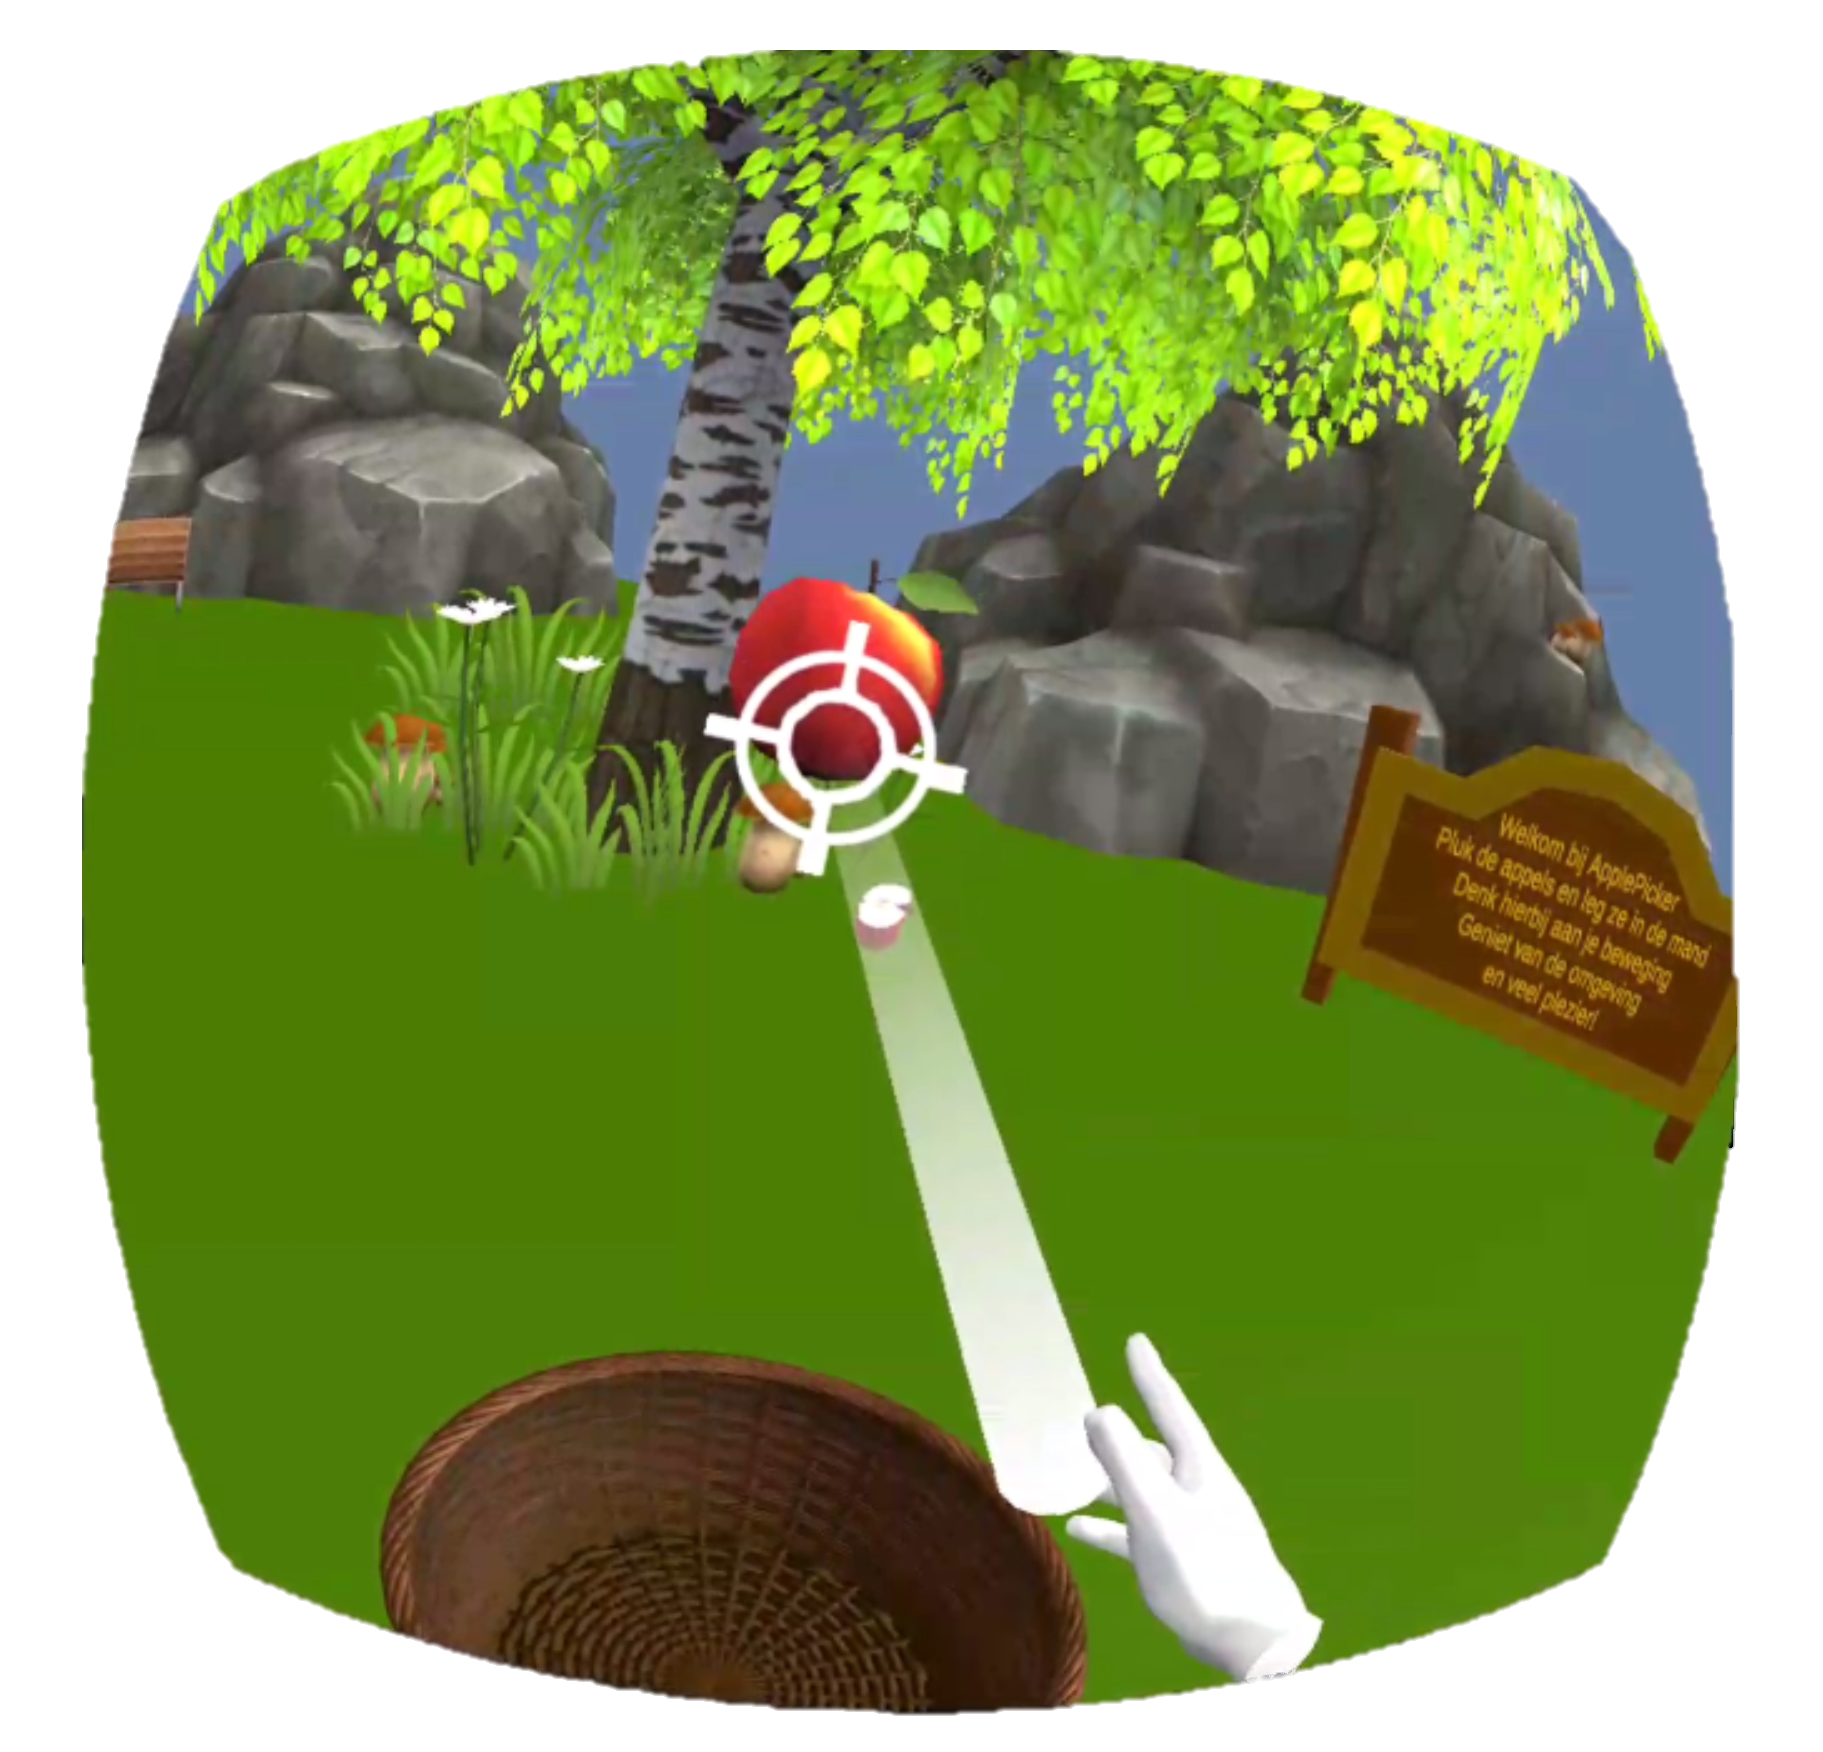
\includegraphics[scale=0.5]{apple3.png}
    \caption{ApplePicker screenshot appel plukken}
\end{figure}

\begin{figure}[h]
    \centering
    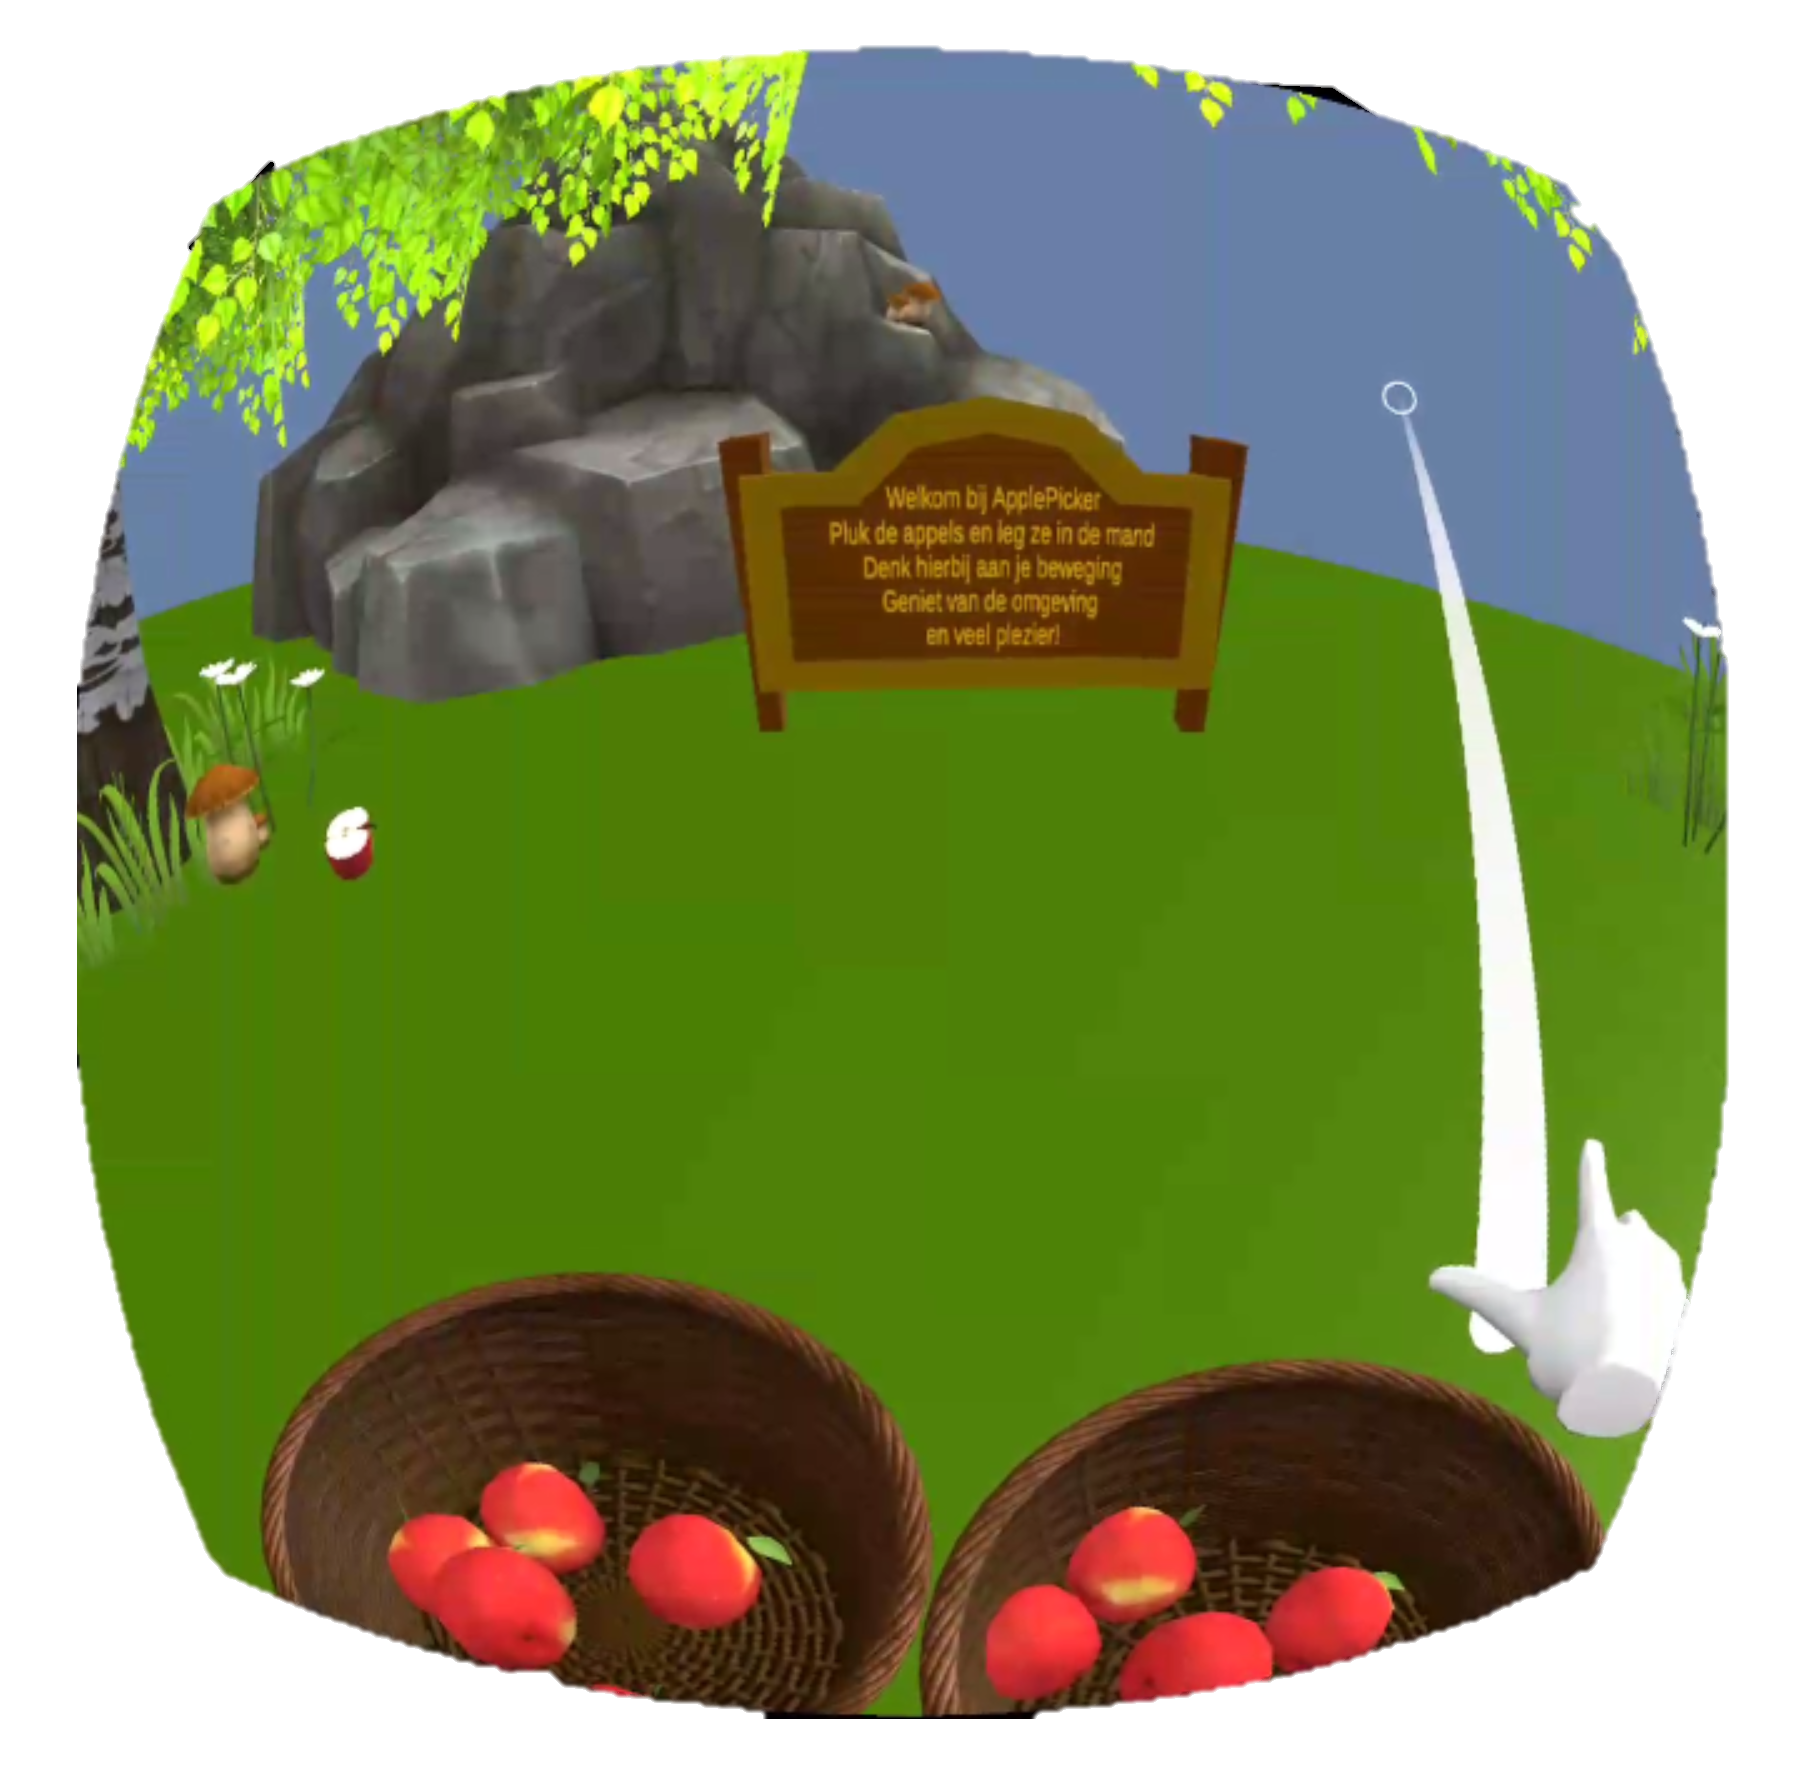
\includegraphics[scale=0.5]{apple4.png}
    \caption{ApplePicker screenshot appels in de manden}
\end{figure}